\documentclass[spanish,a4paper,11pt]{article}

\usepackage[dvips]{graphicx}
\usepackage[dvips]{epsfig}
\usepackage[spanish]{babel}
\usepackage[utf8]{inputenc}
\usepackage{amsmath}
\usepackage{amssymb}


\title{\bf {EL NÚMERO $\pi$}}
\author{Misael Enrique Peraza Luis\\Alumno de Matemáticas de la ULL}
\date{\today}


\begin{document}
\maketitle

\begin{abstract}
El número $\pi$ es bien extraño. No es un número entero, tampoco es un número fraccionario, esto lo deja en la categoría de los números llamados 'irracionales', porque no se puede escribir como una razón entre dos números; a esta categoría pertenecen otros números, $\sqrt{2}$, por ejemplo.
Los números racionales, aunque algunos sean infinitos en su expresión decimal (por ejemplo 1/3 =0.3333…), van a ser periódicos, van a tener una secuencia que se repetirá infinitamente.\textbf{Véase el cuadro \ref{tabla} y la figura \ref{pict}}.
En cambio, los números 'irracionales' son infinitos y no periódicos: la secuencia de decimales nunca termina y además cambia de manera impredecible, hay que ir obteniendo las cifras una a una. \cite{Wpress}
\begin{table}
\centering
\begin{tabular}{lrc}
Número de decimales & $\pi$ \\
\hline
2 & 3.14\\
3 & 3.141\\
4 & 3.1415\\
5 & 3.14159\\
6 & 3.141592\\
\end{tabular}
\caption{El número Pi con sus decimales}
\label{tabla}
\end{table}

\ \\
Además $\pi$ pertenece a un club de números todavía más selecto (al que también pertenece el número $\textbf{e}$): los números trascendentes. Estos ni siquiera pueden ser escritos como la raíz de una fracción, lo que quieres decir que no pueden ser solución de una ecuación algebraica.
A lo largo de la historia, se ha ido buscando y calculando cifras decimales de $\Pi$, en nuestros dias hemos llegado a obtener millones de cifras, empezando por $3.14159…$

Pero, ¿qué decir de $\pi$?, ¿qué es $\pi$?. Quizá la manera más facil de contestar sea que es el resultado de dividir la longitud de la circunferencia entre su diámetro, pero desde luego esto no agota el número $\pi$.

Aparece de manera 'natural' en multitud de fórmulas que explican fenómenos naturales, en casi cualquier campo de las matemáticas, en resumen, en donde menos te lo esperas.

\begin{figure}[!ht]
\centering
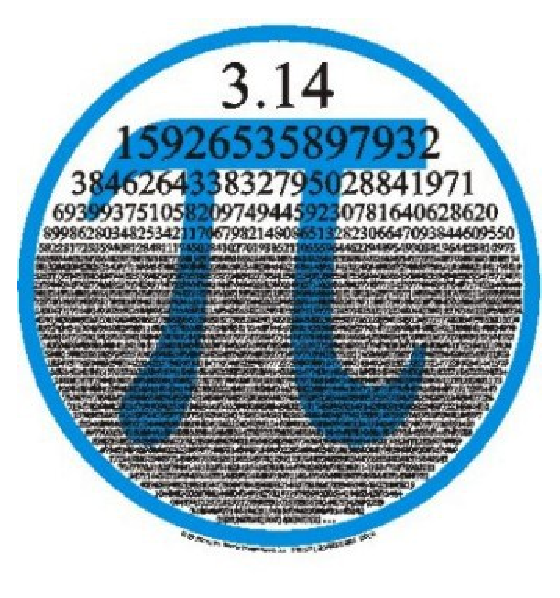
\includegraphics[width=0.5\textwidth]{numpi.eps}
\caption{Número Pi y parte de sus decimales}
\label{pict}
\end{figure}
\end{abstract}

\section {Aproximaciones geométricas a $\pi$}

Es posible obtener una aproximación al valor de $\pi$ de forma geométrica. De hecho, ya los griegos intentaron obtener sin éxito una solución exacta al problema del valor de $\Pi$ mediante el empleo de regla y compás. El problema griego conocido como cuadratura del círculo o, lo que es lo mismo, obtener un cuadrado de área igual al área de un círculo cualquiera, lleva implícito el cálculo del valor exacto de $\pi$.\cite{Wiki}

Una vez demostrado que era imposible la obtención de $\pi$ mediante el uso de regla y compás, se desarrollaron varios métodos aproximados. Dos de las soluciones aproximadas más elegantes son las debidas a Kochanski (usando regla y compás) y la de Mascheroni (empleando únicamente un compás).
\subsection {Método de Kochaski}

Se dibuja una circunferencia de radio R. Se inscribe el triángulo equilátero OEG. Se traza una recta paralela al segmento EG que pase por A, prolongándola hasta que corte al segmento OE, obteniendo D. Desde el punto D y sobre ese segmento se transporta 3 veces el radio de la circunferencia y se obtiene el punto C. El segmento BC es aproximadamente la mitad de la longitud de la circunferencia.
\subsection {Método de Mascheroni}

Método desarrollado por Lorenzo Mascheroni: se dibuja una circunferencia de radio R y se inscribe un hexágono regular. El punto D es la intersección de dos arcos de circunferencia: BD con centro en A', y CD con centro en A. Obtenemos el punto E como intersección del arco DE, con centro en B, y la circunferencia. El segmento AE es un cuarto de la longitud de la circunferencia, aproximadamente.

\section {Historia del cálculo del valor $\pi$}

La búsqueda del mayor número de decimales del número $\pi$ ha supuesto un esfuerzo constante de numerosos científicos a lo largo de la historia. Algunas aproximaciones históricas de $\pi$ son las siguientes.\cite{Wiki}

\subsection{Renacimiento europeo}

A partir del siglo XII, con el uso de cifras arábigas en los cálculos, se facilitó mucho la posibilidad de obtener mejores cálculos para $\pi$. El matemático Fibonacci, en su Practica Geometriae, amplifica el método de Arquímedes, proporcionando un intervalo más estrecho. Algunos matemáticos del siglo XVII, como Viète, usaron polígonos de hasta 393.216 lados para aproximarse con buena precisión a 3,141592653. En 1593 el flamenco Adriaan van Roomen (Adrianus Romanus) obtiene una precisión de 16 dígitos decimales usando el método de Arquímedes.
\subsection{Matemática islámica}

En el siglo IX Al-Jwarizmi, en su Álgebra (Hisab al yabr ua al muqabala), hace notar que el hombre práctico usa 22/7 como valor de $\pi$, el geómetra usa 3, y el astrónomo 3.1416. En el siglo XV, el matemático persa Ghiyath al-Kashi fue capaz de calcular el valor aproximado de $\pi$ con nueve dígitos, empleando una base numérica sexagesimal, lo que equivale a una aproximación de 16 dígitos decimales: 2$\pi$ = 6.2831853071795865.

\footnote{$http://www.facultades.ull.es/Private/folder/centros/matematicas/gradomat/informaciongeneral/mem_grado_matematicas_marzo2010.pdf$}

\begin{thebibliography}{99}
\bibitem{Wiki}
Wikipedia
\bibitem{Wpress}
Wordpress\\
\end{thebibliography}





\end{document}


